\section{Resultados do Estudo de Caso}
\label{sec:resultados}


Os resultados dos dados coletados foram categorizados em três efeitos: entrega de ordens de serviço, satisfação do cliente e qualidade interna do código fonte. É importante destacar que é a partir da análise desses efeitos que responderemos às questões específicas elaboradas para investigar o problema apresentado. 

\subsection[Efeitos sobre a entrega de ordens de serviço]{Efeitos sobre a entrega de ordens de serviço}

A partir dos dados coletados da documentação dos Processos do projeto SICG foram calculadas as métricas para responder as questões específicas QE1 a QE9, que caracterizam os efeitos sobre a entrega de ordens de serviço do uso de métodos ágeis na gestão do contrato de fornecedores de desenvolvimento de \textit{software}.

A Tabela \ref{resultadosmetricas} apresenta os resultados das métricas para cada uma das questões específicas anteriormente mencionadas.


\begin{table}[h]
\footnotesize
\center
\begin{tabular}{|p{0.5cm}|p{5.0cm}|}
\hline
\textbf{ID}                                                                                                                                & \textbf{Resultado da Métrica}    \\ \hline
QE1.                                                                                                          & 25 ordens de serviço          \\ \hline
QE2.                                                                       & 20 ordens de serviço          \\ \hline
QE3.                                                                       & 1 ordem de serviço            \\ \hline
QE4.                                                                                                      & 80\%                          \\ \hline
QE5.                                                                                                  & 3.7 semanas                   \\ \hline
QE6.        & 4 ordens de serviço           \\ \hline
QE7.                                                                                    &  Tabela \ref{porcentagemrequisitos} \\ \hline
QE8.                                                                                                            & 0 multas                      \\ \hline
QE9.                                                                                             & Tabela \ref{custo}                 \\ \hline
\end{tabular}
\caption{Resultados Métrica de QE1. a QE9.}
		\label{resultadosmetricas}
\end{table}


A Tabela \ref{porcentagemrequisitos} apresenta a porcentagem de requisitos atendidos em cada ordem de serviço ou \textit{sprint}, respondendo assim a questão específica QE7.



\begin{table}[h]
\footnotesize
\center
\begin{tabular}{|l|l|l|l|l|l|l|l|l|l|l|l|l|l|l|l|l|l|l|l|l|l|l|l|l|l|}
\hline
\textbf{\textit{Sprint}} & 0   & 1 &  2 & 3 & 4 & 5 & 6 & 7 & 8  \\ \hline
\textbf{OS} & 1 &  2 & 3 & 4 & 5 & 6 & 6.1 & 7 & 8  \\ \hline
\textbf{\% de Requisitos Atendidos} & 100\% &  0\%    & 94\%    & 0\%    & 94\%         & 100\%        & 0\%       & 100\%                                                                                     & 94\%               \\ \hline \hline
\textbf{\textit{Sprint}} &  9 & 10 & 11 & 12 & 13 & 14 & 15 & 16  & -\\ \hline
\textbf{OS} &  9 & 10 & 11 & 12 & 13 & 14 & 15 & 16 & - \\ \hline
\textbf{\% de Requisitos Atendidos} &   100\%                                       & 100\%           & 100\%  & 100\% & 84\%         & 100\%         & 100\%       & 100\%  &-         \\ \hline \hline
\textbf{\textit{Sprint}} &  17 & 18 & 19 & 20 & 21 & 22 & 23 & 24  & -\\ \hline
\textbf{OS} &  17 & 18 & 19 & 20 & 21 & 22 & 23 & 24 & - \\ \hline
\textbf{\% de Requisitos Atendidos} &  84\%        & 0\%        & 100\%          & 100\% & 100\%     & 36\%      & 60\%        & 100\%          &-                                                                          \\ \hline

\end{tabular}
\caption{Porcentagem de Requisitos Atendidos por Ordem de Serviço}
		\label{porcentagemrequisitos}
\end{table}

 A média geral de requisitos atendidos ao longo do projeto de acordo com os dados levantados da documentação foi de 78\%, o que coincide com a percepção dos envolvidos no projeto: 75\% dos envolvidos responderam ao questionário que a percepção geral de requisitos atendidos durante o projeto estava entre 70\% e 90\%.

A Tabela \ref{custo} apresenta o custo de cada ordem de serviço ou \textit{sprint}, respondendo assim a questão específica QE9. Como pode ser observado, nas ordens de serviço que tiverem a porcentagem de requisitos atendidos como 0\% não houve remuneração para a contratada. O custo estimado do contrato antes da contratação era de R\$ 990,000. Portanto, o custo final foi próximo do custo estimado, ultrapassando apenas 1,8\%.

\begin{table}[h]
\footnotesize
\center
\begin{tabular}{|l|l|l|l|l|l|l|l|l|l|l|l|l|l|l|l|l|l|l|l|l|l|l|l|l|l|}
\hline
\textbf{\textit{Sprint}} & 0   & 1 &  2 & 3 & 4 & 5 & 6  \\ \hline
\textbf{OS} & 1 &  2 & 3 & 4 & 5 & 6 & 6.1 \\ \hline
\textbf{Custo}  & R\$                    49,500.00   & R\$                                 0.00   & R\$                    53,316.25    & R\$                                 0.00    & R\$                    36,382.50         & R\$                    31,927.50   & R\$                                 0.00                  \\ \hline \hline
\textbf{\textit{Sprint}}  & 7 & 8 &  9 & 10 & 11 & 12 &-\\ \hline
\textbf{OS}  & 7 & 8 &  9 & 10 & 11 & 12 &- \\ \hline
\textbf{Custo}        & R\$                    45,478.13                                                                                      & R\$                    31,741.88   &   R\$                    29,143.13                                        & R\$                    65,896.88          &  R\$                    64,597.50  & R\$                  107,291.25   &-      \\ \hline \hline
\textbf{\textit{Sprint}} & 13 & 14 & 15 & 16 &  17 & 18  &-\\ \hline
\textbf{OS} & 13 & 14 & 15 & 16 &  17 & 18 &-  \\ \hline
\textbf{Custo}  & R\$                    56,801.25         & R\$                    39,909.38       & R\$                    63,669.38        &  R\$                    61,627.50  &  R\$                    31,185.00        &R\$                                 0.00                                                   &-       \\ \hline \hline
\textbf{\textit{Sprint}} & 19 & 20 & 21 & 22 & 23 & 24&-  \\ \hline
\textbf{OS} & 19 & 20 & 21 & 22 & 23 & 24&- \\ \hline
\textbf{Custo}  &  R\$                    53,831.25  &      50,490.00 & R\$                    63,112.50     & R\$                    13,612.50       & R\$                    22,027.50       &  R\$                    36,630.00 &-                                                        \\ \hline

\end{tabular}
\caption{Custo por Ordem de Serviço}
		\label{custo}
\end{table}


É importante destacar que apesar das \textit{sprints} 1, 3, 6 e 18 não tiverem sido faturadas, não houve aplicação de multa para a contratada. Pois, conforme a solução caracterizada anteriormente, o órgão optou por modificar o modelo de remuneração e considera o aprendizado e a adaptação da empresa ao tipo de metodologia de gestão de contrato que está sendo aplicado. Além disso, o fato de a empresa não ter um pagamento em seu fluxo de caixa já é penalização suficiente para que a empresa faça a adequação do seu processo de trabalho.

Outro fato importante é que ao entregar uma ordem de serviço para homologação, uma recontagem de pontos por funções do que foi entregue era realizada, e ao realizar a homologação o fiscal técnico do IPHAN realizava uma nova contagem de pontos por função sobre as funcionalidades homologadas. Apenas o valor de pontos de função das funcionalidades homologadas eram faturados. 

Ainda, pelos dados coletados neste estudo, não foi evidenciada a utilização de uma técnica de gerenciamento de custos do projeto, como exemplo, o valor agregado. Uma ferramenta que automatize o processo de acompanhamento de custos poderia prover uma informação mais adequada e poderia auxiliar o gestor na tomada de decisão. O gestor do contrato poderia analisar, por exemplo, se o que está sendo pago está de acordo com o que está sendo produzido ou de acordo com o que foi planejado.

\subsection[Efeitos sobre a satisfação do cliente]{Efeitos sobre a satisfação do cliente}

O cliente do projeto SICG é representado pelo papel de \textit{Product Owner}, que também atuou como gestor do contrato, e por todos os envolvidos no projeto por parte do IPHAN. Este nunca havia participado anteriormente de um projeto onde a gestão do contrato era realizada com o uso de métodos ágeis, portanto, a experiência dos envolvidos no projeto com esses métodos era pouca. Para coletar a opinião do cliente acerca das questões específicas QE10  e QE11 foi aplicado o questionário encontrado no Apêndice A.

A Figura \ref{visibilidade} apresenta a visibilidade do processo de todos os envolvidos no projeto por parte do IPHAN. Cerca de 80\% dos envolvidos no projeto considerou a visibilidade do processo como "Alta", dentre eles o gestor do contrato. A Figura \ref{satisfacao} apresenta o resultado de satisfação do IPHAN com relação ao produto entregue. De forma unânime foi considerado como "Satisfeito" o produto entregue pela empresa contratada. 


\begin{figure}[h]
\subfigure[visbilidade] [Nível de Visibilidade do Processo do Projeto SICG]{
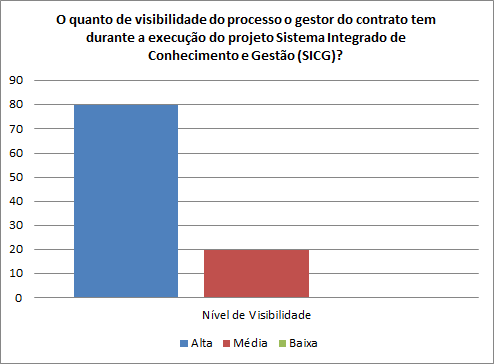
\includegraphics[scale=0.6]{figuras/visibilidade.png} \label{visibilidade}}
\subfigure[satisfacao] [Nível de Satisfação do Produto Entregue do Projeto SICG]{
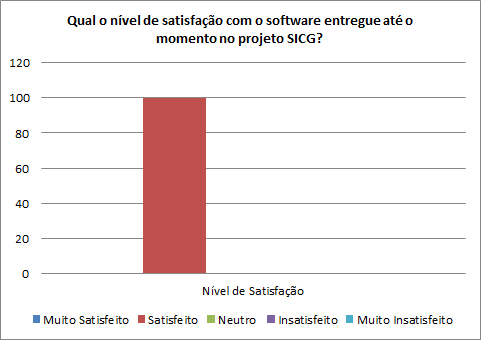
\includegraphics[scale=0.6]{figuras/satisfacao.png} 	\label{satisfacao}}
\end{figure}



\subsection[Efeitos sobre a qualidade do código]{Efeitos sobre a qualidade do código}

Para cada uma das \textit{sprints} do SICG, coletou-se o código fonte disponibilizado pelo IPHAN. A qualidade do código fonte do SICG pode ser avaliada por meio de métricas que evidenciam a qualidade externa \cite{ISO25023}. Neste trabalho foram selecionadas doze métricas de código fonte levantadas e categorizadas em: métricas de tamanho e complexidade e métricas de orientação à objetos \cite{Meirelles2013}. 


Um dos objetivos científicos do estudo de Meirelles foi a identificação das distribuições estatísticas dos valores das métricas apresentadas anteriormente em 38 projetos de \textit{software} livre, onde foram analisadas 344.872 classes das aplicações mais utlizadas de \textit{software} livre, tais como, Chrome, Firefox, OpenJDK e VLC. A partir de cada uma das distribuições estatísticas foram classificadas as métricas de código fonte de acordo com a frequência dos valores apresentados,
com os intervalos: muito frequente, frequente, pouco frequente e não frequente. Para simplificar o entendimento das métricas de código fonte, Morais interpretou os rótulos dos
intervalos de frequência definidos por Meirelles em em rótulos qualitativos: excelente, bom, regular e ruim.


Os intervalos utilizados para se chegar as esses indicadores de qualidade foram retirados do
estudo de Meirelles, para esse trabalho foram utilizados os intervalos encontrados para C++ e Java. É importante ressaltar que quando apresentarmos o resultado da análise sobre o código fonte deste estudo de caso e dissermos que o código fonte tem um rótulo "Excelente" ou "Ruim" para determinada métrica, siginifica dizer que, esse código fonte é "Excelente" ou "Ruim" em comparação ao melhor projeto de \textit{software} livre selecionado por Meirelles na Linguagem Java, que foi o Open JDK8.



De forma geral, o processo realizado para a análise do código fonte do SICG consistiu em: i) executar a ferramenta de análise estática de código fonte, Analizo, sobre o código fonte do projeto SICG; ii) Após o passo i o resultado será armazenado em um arquivo .csv \footnote{Comma-separated values (ou CSV) é um formato de arquivo que armazena dados tabelados} com as medidas númericos das métricas selecionadas; iii) transformar o arquivo .csv em json\footnote{JSON (JavaScript Object Notation) é um modelo para armazenamento e transmissão de informações no formato texto, tem sido bastante utilizado por aplicações Web devido a sua capacidade de estruturar informações de uma forma bem mais compacta, tornando mais rápido o parsing dessas informações.} ; iv) e por fim, processar esse arquivo em uma solução desenvolvida em um ambiente de Datawarehousing, utilizando a ferramenta Pentaho. Ao final desse processo, temos como resultado os gráficos para análise. 

A fim de responder a questão específica QE12 são mostrados a seguir os resultados do processamento do código fonte do projeto SICG no que diz respeito a qualidade interna do produto ao longo das \textit{sprints} do projeto, 
de acordo com as 12 métricas selecionadas: LOC (Lines of Code), ACCM (Average Cyclomatic Complexity per Method), AMLOC (Average Method Lines of Code), ACC (Afferent Connections per Class), ANPM (Average Number of Parameters per Method),
CBO (Coupling Between Objects), DIT(Depth of Inheritance Tree), LCOM4 (Lack of Cohesion in Methods), NOC (Number of Children), NOM (Number of Methods), NPA (Number of Public Attributes) e RFC (Response For a Class).

Foram identificados cenários de limpeza de código fonte a partir dos resultados das métricas citadas anteriormente. Dentre os tipos de cenários de limpeza identificados os mais incidentes foram: 
Compexidade Estrutural, Classe Pouco Coesa e Interface dos Métodos. Outros tipos de cenários de limpeza como Classe com Muita Exposição, Classe
com Muitos Filhos e Classe com Método Muito Grande também foram identificados, porém, com menos frequência.

Dentre esses cenários identificados, o cenário de limpeza de código fonte Complexidade Estrutural é aquele que o tratamento deveria
ser priorizado, pois ele correspondeu de 55\% a 68\% da quantidade total de cenários identificados.

A \textit{Sprint} 24 é a última \textit{sprint} do projeto e, portanto, é nela que foi entregue o código fonte final. Conforme a Fig. \ref{pizzatotal}, na análise da qualidade do código fonte dessa \textit{sprint}, observamos uma predominância do intervalo de qualidade "Excelente", o qual acontece em 7 métricas. O intervalo de qualidade "Bom" acontece em 3 métricas. O intervalo de qualidade "Regular" acontece em 1 métrica. E o intervalo de qualidade "Ruim" acontece em 1 métrica.

\begin{figure}[h]
		\centering
			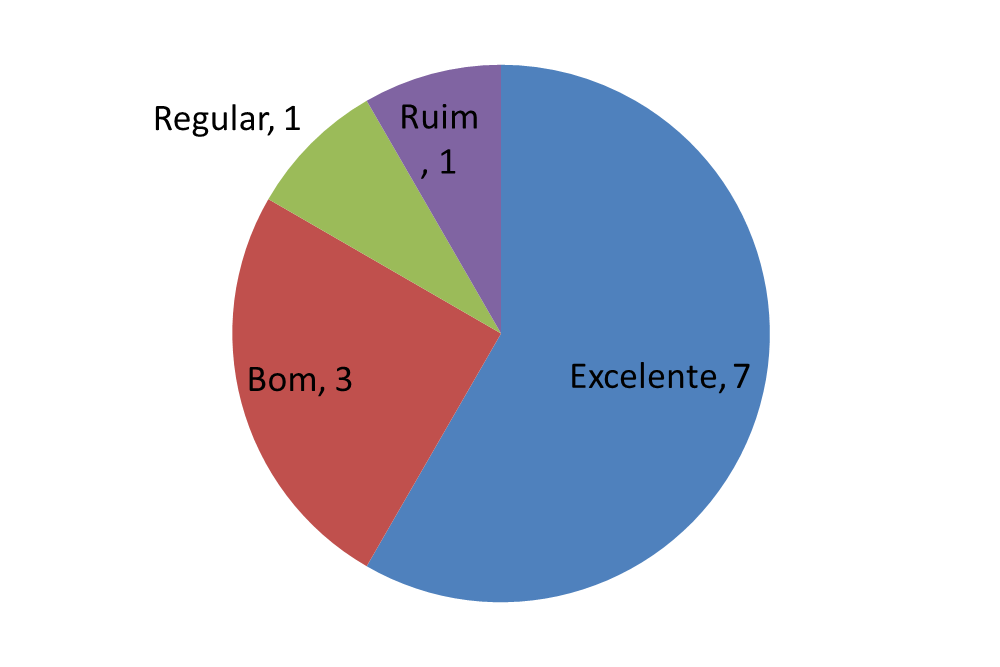
\includegraphics[scale=0.5]{figuras/pizzatotal.png}
		\caption{Qualidade Geral do Código Fonte}
		\label{pizzatotal}
\end{figure}


Foi analisada ainda a percepção da qualidade do código fonte do SICG segundo os envolvidos no projeto (Scrum Master, Product Owner, Gestor do Contrato, Coordenador do Projeto, Fiscal Técnico e Desenvolvedores). Como ilustrado na figura \ref{percepcaoqualidade}, cerca de 66\% dos envolvidos consideraram  o intervalo de qualidade do código como "Excelente" e os demais consideraram
o intervalo de qualidade como "Bom".

\begin{figure}[h]
		\centering
			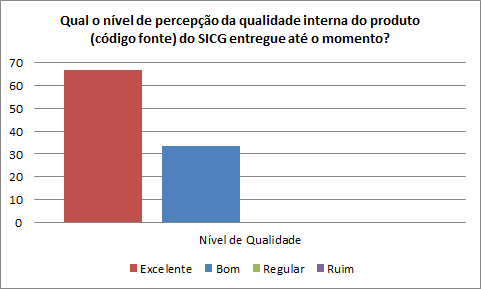
\includegraphics[scale=0.7]{figuras/percepcaoqualidade.png}
		\caption{Nível de Percepção da Qualidade do Código Fonte}
		\label{percepcaoqualidade}
\end{figure}

Assim, no que diz respeito a análise estática do código realizada, a qualidade interna do produto pode ser considerada satisfatória ao compararmos com o melhor \textit{software} livre encontrado na linguagem de programação Java, retirado do estudo de Meirelles. Além disso, há uma convergência com a também percepção satisfatória na dos envolvidos no projeto SICG, embora não tenhamos encontrado evidências de que o IPHAN realizava análise sistemática sobre tais métricas de qualidade de produto.

O fato de padrões de qualidade de métricas de código fonte não terem sido específicados no contrato e o fato de uma análise de qualidade de código de fonte não ter sido realizada durante os ciclos do projeto figuraram como risco ao projeto, uma vez que poderia ter comprometido o sucesso e a manutenibilidade do sistema. Al[em disso, não evidenciamos a entrega de uma suíte de testes automatizada, o que poderia ter aumentado a qualidade interna do produto assim como sua segurança e robustez no ateste técnico de uma ordem de serviço.